\chapter{Design \& Implementation} \label{chap:design}


This chapter introduces the concept of the data-processing framework for OVD (Section 4.1). 
Section 4.2 proposes a software, which is designed for this framework.
The rest described the individual modules within the proposed framework in details (Section 4.3, 4.4, 4.5, 4.6).

This chapter present the design and implementation for our OVD software project.
Section \ref{chap:design:overview} provides an overview for the software design, which comprises of separated modules.
These modules will be explained further in the subsequent sections.
Finally, we introduce a setup based on the framework to demonstrate a complete workflow in Section \ref{chap:design:software} \mtd{improve}
% The rest described the individual modules within the proposed framework in details (Section 4.3, 4.4, 4.5, 4.6).


\section{Framework Overview}\label{chap:design:overview}
The framework is designed to be self-contained, easy to utilize and maintain, yet capable of being scaled out to sorts of OVD.
To achieve these goal, we decide to split the software logic into modules, each is isolated in compartment, or \textit{module}.
These modules are self-contained, stand-alone software programs that run on any POSIX environment (Linux, macOS).
A single module is responsible for a stage in the OVD data process: making raw data available, cleaning data from abnormal values, storing in  centralized database in a pre-defined format, as well as extracting meaningful data using scientific methods.
To ensure portability and scalability, we decide to package the modules in software container using Docker along with a Docker-compose script for quick deployment.
However, for horizontal scale up, these independent containers can be deployed in a Kubernetes cluster \mtd{improve}.


% The data-processing framework is designed to handle large-scale, time-series operational vessel data (OVD), facilitating the transformation of raw data into presented insights.
The proposed framework (Figure \ref{fig:design:framework-overview}) composes of four modules, corresponding to four common stages in data engineering: data collection, data cleaning, data storage, data presentation. 
By decoupling the logics, the framework can be extended by adding new module in between existing modules. 
Additionally, the processing capacity of each stage can be scaled by running many containers simultaneously with the same logic scripts \mtd{improve this}.
For management and interaction purpose, each module is provided with a user interface (called "Module management").

\begin{figure}[H]
    \centering
    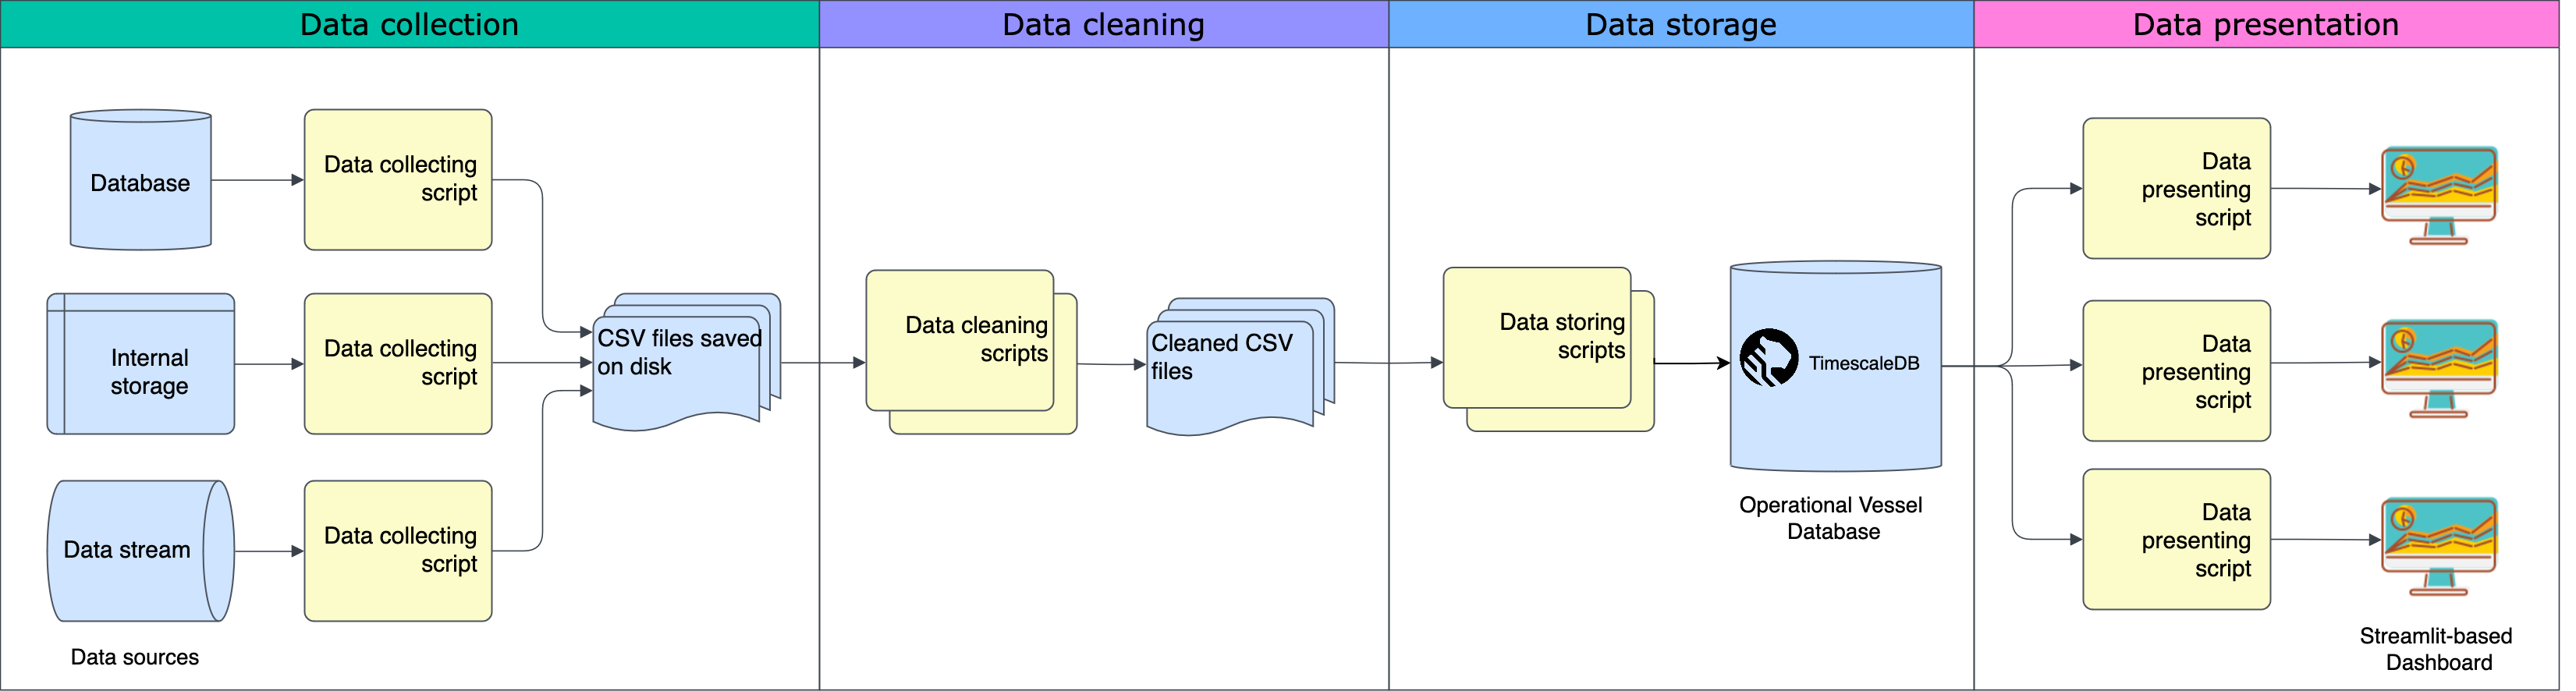
\includegraphics[width=1.0\linewidth]{studentWorkTemplate_en/figures/mt-222100012-framework-overview.drawio.png}
    \caption{The proposed framework for OVD}
    \label{fig:design:framework-overview}
\end{figure}

Starting from the left of Figure \ref{fig:design:framework-overview}, the data collection module is tasked with collecting data automatically from various user-defined data sources. By running collecting scripts periodically, every data sources are saved to the hard disk under CSV format. 
Subsequently, the cleaning module allows user to choose a CSV file on disk and a suitable cleaning script. Then, the module run the cleaning script, which clean the data file and return the cleaned data file to the hard disk (also under CSV format). 
Similarly, the data storage module once again run the selected storing script on the selected cleaned data file to save it to TimescaleDB for long term uses. 
At the last module, the data from TimescaleDB database will be retrieved and computed by dashboards, which ensure the visualization is intuitive and interactive to users.


\begin{figure}[H]
    \centering
    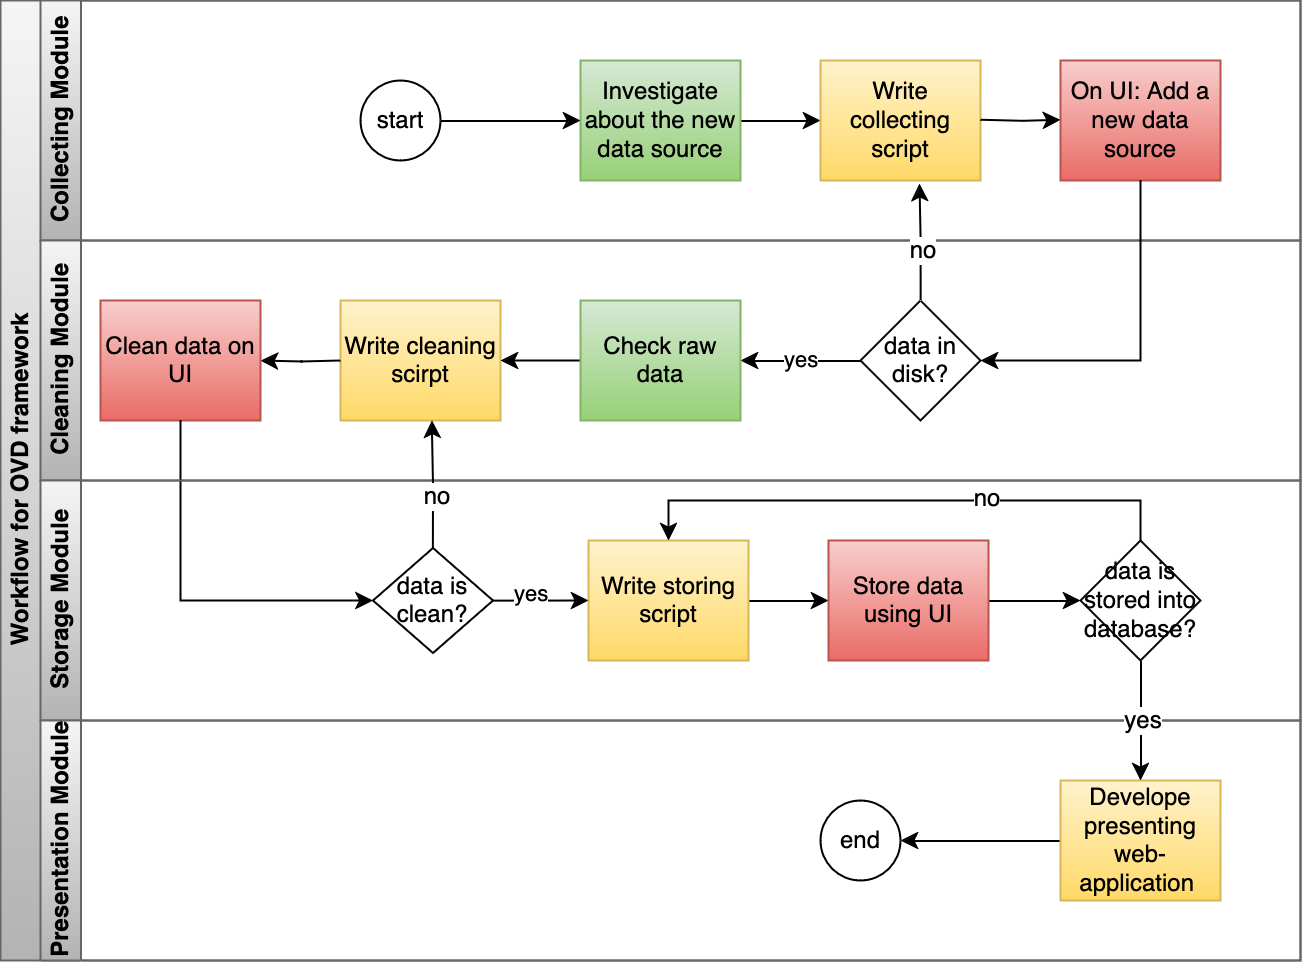
\includegraphics[width=0.8\linewidth]{studentWorkTemplate_en/figures/mt-222100012-workflow.drawio.png}
    \caption{Workflow for user}
    \label{fig:framework-workflow}
\end{figure}

To view the framework from user perspective, Figure \ref{fig:framework-workflow} presents step-by-step workflow. 

\section{Implementation overview}
\label{chap:design:software}
Along with the proposed framework, we implemented a software to manage and conduct works on the framework more efficiently. 
The framework software is implemented in Python programming language, and can be run on different operating systems. The software is also split to four modules corresponding to four modules of the data-processing framework: data collecting module, data cleaning module, data storage module and data presentation module. Each module has "Module Management" component and Backend component (i.e., data collector, cleaner, integrator, computer). "Module Management" components are a Streamlit-based website, allow user to work with these module. The logic of each module is located at its Backend component.
There are data sharings among modules, which creates the mutual communication and continuity between modules. To facilitate the technical requirement, Docker container and Docker volume are employed to this software. 
The whole system architecture is depicted in Figure \ref{fig:software-architecture}


\begin{figure}[H]
    \centering
    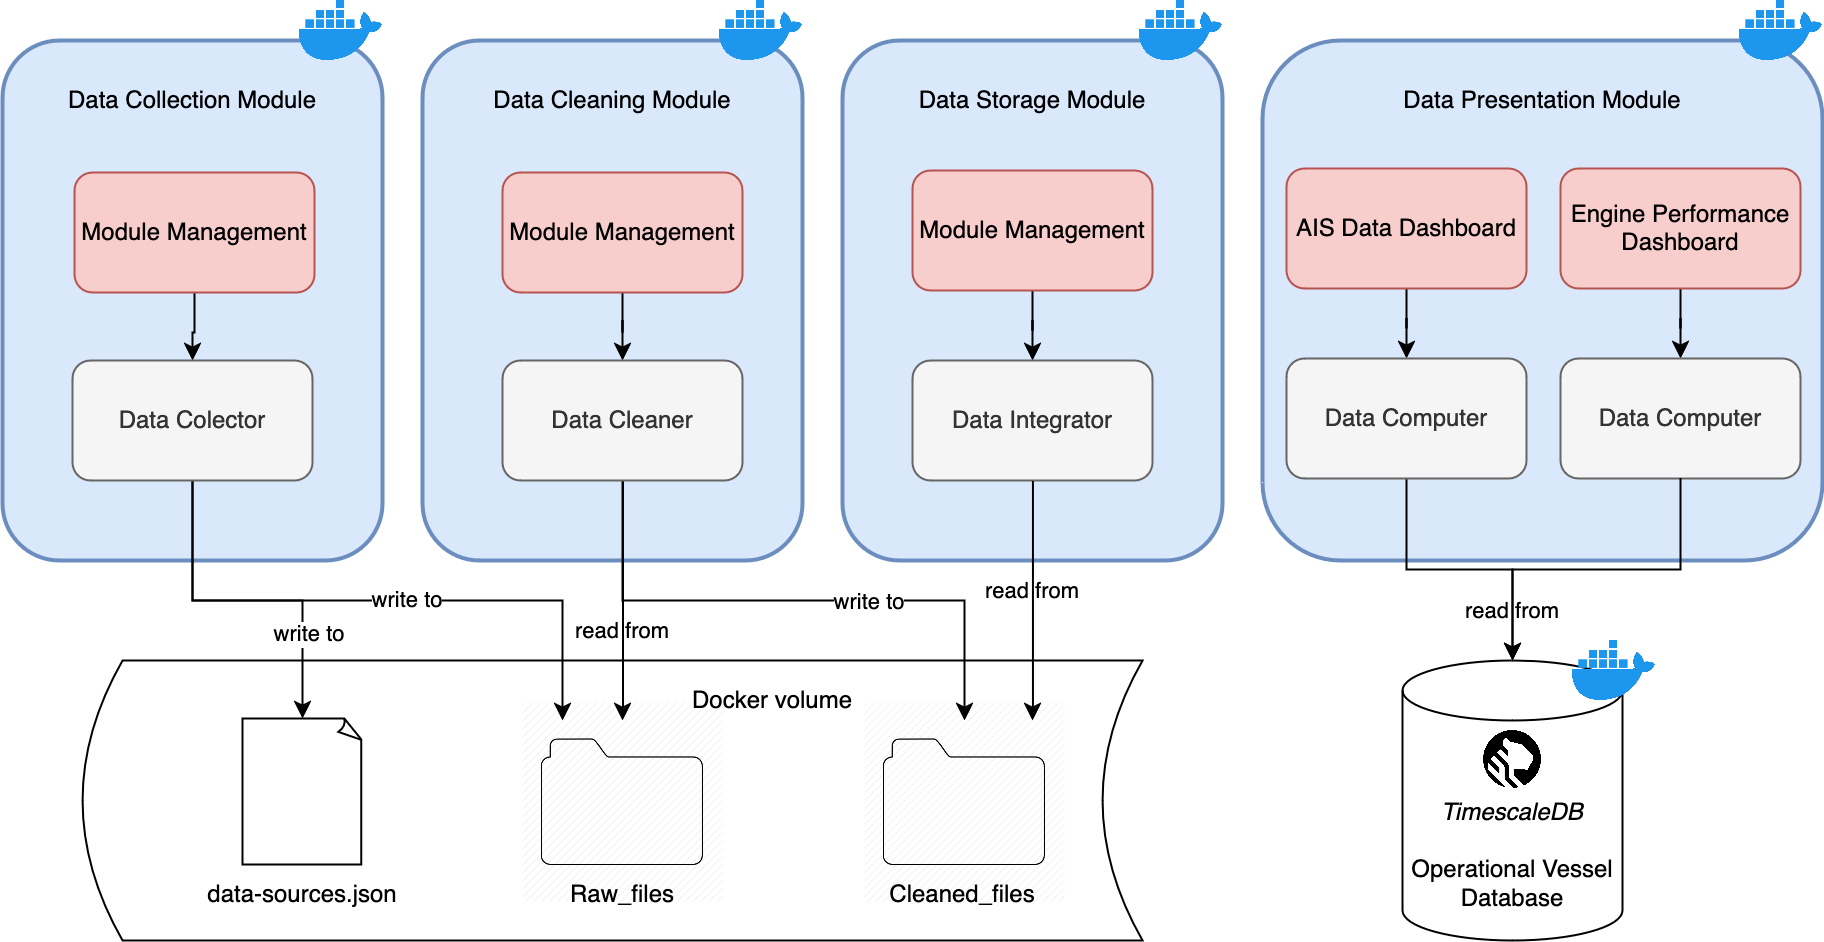
\includegraphics[width=1.0\linewidth]{studentWorkTemplate_en/figures/mt-222100012-system-architecture.drawio.png}
    \caption{Docker deployment}
    \label{fig:software-architecture}
\end{figure}

\mtd{1 para why you choose Docker container? why you choose Docker volume?}
Setting up with Docker, the software utilizes the portable and stable characteristics of Docker, help it deploy more easily. Docker Volume is used to keep up-to-dated of code and data files across the four Docker containers. 
The database, which is used for this framework is TimescaleDB, is also containerized and be access via TCP protocol. 

\mtd{Screenshot of one of four "Module Management" }


\section{Module 1: Data collection}
\mtd{write down here objectives of data collection module}

\subsection{Overview}
The primary goal is to gather raw data from various sources (databases, APIs, etc.) in a convenient and flexible manner. Additionally, the captured data should be comprehensive, complete to support downstream processing.
From the UI, user can monitor the amount of raw data 

At first, the data collection module saves information about data sources given by user to data-sources.json. 
For user, the module's frontend enables add, delete and edit a data source. Meanwhile in the backend, the data collector accesses data source periodically, download data and convert to CSV format, saved to the local disk.

\subsection{Workflow}
\mtd{ghi ro rang: nguoi dung cung cap script, chon url, chon cho luu, thiet lay chay lap lai may ngay mot lan, ...}

\subsection{Software Implementation}
\mtd{API server, Python runner, Streamlit, ...}

\subsection{Deployment}
\mtd{Yeu cau: port mo, docker volume, stateless for scaling. Module nay noi chuiyne voi cac modulke khac nhu the nao, voi nguoi dung nhu the nao (web, cmd line, api, ...)}
\mtd{du lieu luu o dau (path) trong container, va ben nguoi host, permission for data to access from host}

\subsection{Saving data sources}
\mtd{move to implementation}
Each data source is saved with attributes

\begin{longtable}{|c|p{4cm}|p{8cm}|}
    \hline
    \textbf{Index} & \textbf{Attribute} & \textbf{Description} \\ \hline
    \endfirsthead
    \multicolumn{3}{c}%
    {{\bfseries Table continued from previous page}} \\
    \hline
    \textbf{Index} & \textbf{Attribute} & \textbf{Description} \\ \hline
    \endhead
    \hline \multicolumn{3}{|c|}{{Continued on next page}} \\ \hline
    \endfoot
    \hline
    \endlastfoot

    1 & Source Name & The name of the data source or system providing the data. \\ \hline
    2 & Source URL & The URL or endpoint where the data can be accessed. \\ \hline
    3 & Source Description & A brief description of the data source and what kind of data it provides. \\ \hline
    4 & File Format & The format in which the data is provided or stored (e.g., CSV, JSON). \\ \hline
    5 & Collecting Script & The script or method used to collect the data (e.g., Python script, API call). \\ \hline
    6 & Category & The category of the data source (e.g., sensor data, weather data). \\ \hline
    7 & Collecting Frequency & The frequency at which the collecting script is scheduled to run by the system (Every minute, Hourly, Dayly, Weekly, Monthly). \\ \hline

\end{longtable}
This is an example of 2 data sources saved json file:

\begin{verbatim}
[
    {
        "name": "[AIS Hub] csv",
        "url": "sdf",
        "description": "sdfsdfsdf"
    }
]
\end{verbatim}

\section{Module 2: Data cleaning}
\subsection{Overview}
\mtd{write down here objectives of this data cleaning module}
This module allows user to choose the data file and its cleaning scripts to clean processing.
With one script, one cleaning procedures but can reused for different file. It will reduce time for this cleaning task.

\subsection{Eliminate common errors in OVD}
This is some common errors occurred in OVD.


\begin{table}[]
\begin{tabular}{|l|l|l|}
\hline
\textbf{Category} & \textbf{Error} & \textbf{Example} \\ \hline
Column-related errors & wrong column names & abcd \\ \hline
 & wrong column data type &  dbe \\ \hline
 & wrong column data format & xyz \\ \hline
 &  &  \\ \hline
Row-related errors & missing row & \begin{tabular}[c]{@{}l@{}}Depends on the requirements: \\ ignore, or mark for post processing\end{tabular} \\ \hline
 & duplicated row & Detect duplication and remove on needed \\ \hline
 & consecutive rows are inconsistent & Detect by comparison and -remove/edit \\ \hline
 &  &  \\ \hline
\begin{tabular}[c]{@{}l@{}}Corrupted\\ cell's content\end{tabular} & NaN, null, Unknown values & Depends on requirements: remove rows, or mark. \\ \hline
 & miss-typed values & Replace with the correct values or remove that row \\ \hline
 & outlier values: too high, to low values & Remove that row \\ \hline
 & wrong timestamp & Remove that row \\ \hline
 &  &  \\ \hline
\end{tabular}
\end{table}


\subsubsection{Error 1.1}

\subsubsection{Error 1.2}

\section{Module 3: Data storage}
\subsection{Overview}

\subsection{Database schema}
\mtd{list all popular fields in OVD}
After investigate various sources of OVD data, it is true that the number of fields collected on-board are vast and diverse. Many of them have very less meaningful to save. THerefore, the thesis propose here common and valuable fields for analysis purpose.




As stated in requirements, when a new field come the database will be able to add that field to schema. But when saving the data to the database, the naming should be critical.

\subsection{Database engine: TimescaleDB}
\mtd{1 para why choose this database instead of other databases?}
\mtd{how to set up database}
\subsubsection{Timestamp}
Every point stored in InfluxDB has an associated timestamp. Timestamp has multiple format: UTC, unix. The timestamp for InfluxDB's data point is in nanosecond-precision Unix time.
Therefore, timestamp from every dataset must be transfer to unix format before storing to the database.

\section{Module 4: Data presentation}
Data presentation module is responsible for presents data.
\subsection{Objective}
\subsection{Data Computer}
\mtd{what is data computer? why it is necessary? }
\mtd{ what do you compute? }
\subsection{Dashboard}




